% !TEX program = xelatex
\documentclass[UTF8,fontset=fandol,a4paper,11pt]{ctexart}
\usepackage[margin=21mm,top=23mm,bottom=22mm,headheight=16pt]{geometry}
\usepackage{amsmath,amssymb,mathtools,bm}
\usepackage{tikz}
\usetikzlibrary{arrows.meta,calc,angles,quotes,patterns}
\usepackage{xcolor,booktabs,array,longtable,enumitem,fancyhdr,needspace}
\usepackage[unicode,hidelinks]{hyperref}
\definecolor{ink}{HTML}{24343C}
\definecolor{accent}{HTML}{166A70}
\definecolor{muted}{HTML}{65747A}
\definecolor{rulegray}{HTML}{D4DDE0}
\definecolor{warm}{HTML}{966037}
\color{ink}
\setlength{\parindent}{2em}
\setlength{\parskip}{4pt}
\linespread{1.12}
\AtBeginDocument{\setlength{\abovedisplayskip}{6pt plus 2pt minus 1pt}
\setlength{\belowdisplayskip}{6pt plus 2pt minus 1pt}
\setlength{\abovedisplayshortskip}{0pt plus 1pt}
\setlength{\belowdisplayshortskip}{4pt plus 1pt}}
\setlist[enumerate]{label=(\arabic*),leftmargin=2.3em,itemsep=3pt,topsep=4pt}
\setlist[itemize]{leftmargin=2em,itemsep=2pt,topsep=4pt}
\allowdisplaybreaks[1]
\setlength{\emergencystretch}{2em}
\setcounter{secnumdepth}{0}
\providecommand{\tightlist}{\setlength{\itemsep}{0pt}\setlength{\parskip}{0pt}}
\ctexset{section={format=\Large\bfseries\color{accent},beforeskip=10pt,afterskip=9pt},
subsection={format=\normalsize\bfseries\color{accent},beforeskip=10pt,afterskip=4pt},
subsubsection={format=\normalsize\bfseries,beforeskip=8pt,afterskip=3pt}}
\pagestyle{fancy}
\fancyhf{}
\fancyhead[L]{\small\color{muted}物理学难题集萃}
% 页眉仅保留书名；版本名称只在封面显示。
\fancyfoot[L]{\small\color{muted}\chapterlabel}
\fancyfoot[R]{\small\thepage}
\renewcommand{\headrulewidth}{0.4pt}
\renewcommand{\footrulewidth}{0pt}
\newcommand{\dd}{\mathop{}\!\mathrm{d}}
\newcommand{\vect}[1]{\bm{#1}}
\newcommand{\tagline}[1]{\noindent{\small\color{muted}#1}\par}
\newcommand{\result}[1]{\begin{equation*}\boxed{#1}\end{equation*}}
\newcommand{\figcaption}[1]{\par\vspace{2pt}{\small\color{muted}#1}\par}
\newcommand{\teach}[2]{\Needspace{4\baselineskip}\subsection*{讲解要点与追问}#1\par\smallskip\noindent\textbf{追问：}#2\par}
\newcommand{\workarea}{\par\vspace{7mm}\noindent{\small\color{muted}作答区}\par\vspace{4mm}
\noindent\textcolor{rulegray}{\rule{\linewidth}{0.3pt}}\par\vspace{16mm}
\noindent\textcolor{rulegray}{\rule{\linewidth}{0.3pt}}\par\vspace{16mm}
\noindent\textcolor{rulegray}{\rule{\linewidth}{0.3pt}}\par\vspace{16mm}
\noindent\textcolor{rulegray}{\rule{\linewidth}{0.3pt}}}
\tikzset{axis/.style={-{Stealth[length=2mm]},thin,color=muted},
motion/.style={-{Stealth[length=2.3mm]},thick,color=accent},
force/.style={-{Stealth[length=2.3mm]},thick,color=warm},
traj/.style={thick,color=accent},guide/.style={dashed,thin,color=muted},
object/.style={thick,color=ink},every node/.style={font=\small}}

\newcommand{\edition}{学生版}
\newcommand{\chapterlabel}{第三章\quad 功、能和动量}
\hypersetup{pdftitle={第三章 功、能和动量·学生版},pdfauthor={},pdfsubject={第三章第1--39题}}
\begin{document}
\pdfbookmark[0]{第三章 功、能和动量}{cover}
\thispagestyle{empty}
\vspace*{20mm}
\noindent{\Huge\bfseries 物理学难题集萃}\par\vspace{8mm}
\noindent{\LARGE 第三章\quad 功、能和动量}\par\vspace{10mm}
\noindent{\Large\color{accent}学生版}\par\vspace{8mm}
\noindent\textcolor{accent}{\rule{\linewidth}{1pt}}\par\vspace{8mm}
\noindent 第 1--39 题\par\vspace{5mm}
\noindent 题目、题图与作答区。\par
\vfill
\clearpage
\pdfbookmark[1]{题目目录}{contents}
\section*{题目目录}
\begin{longtable}{@{}>{\color{accent}\bfseries}r p{120mm}@{}}
\toprule 题号 & 题目\\\midrule
\endfirsthead
\toprule 题号 & 题目（续）\\\midrule
\endhead
1 & 撤去下挂物后的弹簧最大速度 \\
2 & 带摩擦水平弹簧振子的过原点条件 \\
3 & 斜面摩擦中动能等于势能的位置 \\
4 & 桌孔下落绳的速度与位置 \\
5 & 单摆碰钉后的完整圆周与撞钉条件 \\
6 & 圆环双球下滑与悬线张力 \\
7 & 滑杆脱离约束后的落点 \\
8 & 轻杆小球跌落与触地速度 \\
9 & 绳绕钉运动与碰钉条件 \\
10 & 引力追及中的最大间距 \\
11 & 地球直通隧道中的运动 \\
12 & 旋转杆上双弹簧小球 \\
13 & 旋转圆环中的平衡稳定性 \\
14 & 弹性小球与移动墙壁 \\
15 & 三质点绳系冲量 \\
16 & 炮弹最高点爆炸 \\
17 & 平板车上多人跳离 \\
18 & 下滑木块中支持力做功 \\
19 & 半圆槽中小球与木块 \\
20 & 非弹性碰撞后弹簧带起木块 \\
21 & 滑块弹簧与断绳条件 \\
22 & 两球与墙的碰撞次数 \\
23 & 三球铰链杆释放 \\
24 & 小球反复弹跳总时间 \\
25 & 台阶逐级弹跳 \\
26 & 固定斜面碰撞反弹 \\
27 & 可动斜面上的斜碰 \\
28 & 相对平板的反射定律 \\
29 & 小球在可动圆环内反射 \\
30 & 三质点万有引力相对平衡 \\
31 & 等功跳车的动能比较 \\
32 & 子弹射入弹簧连接木块 \\
33 & 箱中滑块多次碰撞 \\
34 & 核反应阈能 \\
35 & 变质量物体方程 \\
36 & 下落绳子的变质量分析 \\
37 & 火箭竖直发射 \\
38 & 小球带绳竖直上抛 \\
39 & 雾中水滴变质量下落 \\
\bottomrule\end{longtable}


\clearpage

\pdfbookmark[2]{第 1 题 撤去下挂物后的弹簧最大速度}{q1}

\section*{第 1 题\quad 撤去下挂物后的弹簧最大速度}

\tagline{M-03-01}

劲度系数为 $k$ 的轻弹簧下端竖直悬挂质量分别为 $m_1,m_2$ 的两物体。平衡后突然撤去下方的 $m_2$，撤去过程不给 $m_1$ 冲量。求 $m_1$ 随后运动的最大速率。

\begin{center}\begin{minipage}{\linewidth}\centering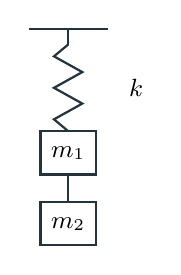
\begin{tikzpicture}
\draw[object] (-.5,3)--(.5,3);\draw[object] (0,3)--(0,2.8);
\draw[object] (0,2.8)--(-.18,2.65)--(.18,2.45)--(-.18,2.25)--(.18,2.05)--(-.18,1.85)--(0,1.7);
\filldraw[object,fill=white] (-.35,1.15) rectangle (.35,1.7);\node at (0,1.42) {$m_1$};\draw[object] (0,1.15)--(0,.8);\filldraw[object,fill=white] (-.35,.25) rectangle (.35,.8);\node at (0,.52) {$m_2$};\node[right] at (.65,2.25) {$k$};
\end{tikzpicture}
\figcaption{图 3.1\quad 撤去下挂物前的平衡状态。}
\end{minipage}\end{center}

\workarea

\clearpage

\pdfbookmark[2]{第 2 题 带摩擦水平弹簧振子的过原点条件}{q2}

\section*{第 2 题\quad 带摩擦水平弹簧振子的过原点条件}

\tagline{M-03-02}

水平轻弹簧一端固定，另一端连接质量为 $m$ 的小球，劲度系数为 $k$。小球在粗糙水平面上运动，静、动摩擦系数均为 $\mu$。弹簧原长位置为 $O$。从右侧 $OA=l_0$ 的 $A$ 点静止释放。
\begin{enumerate}\item 为使小球穿过 $O$ 且只穿过一次，$\mu$ 应取什么范围？以速度不为零并越到另一侧为“穿过”。\item 若还要求小球在左侧第一个转折点 $B$ 永久停住，$OB=l_1$ 的最大值是多少？\end{enumerate}

\begin{center}\begin{minipage}{\linewidth}\centering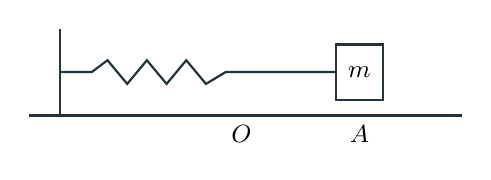
\begin{tikzpicture}
\draw[object] (-.4,0)--(5.1,0);\draw[object] (0,0)--(0,1.1);\draw[object] (0,.55)--(.4,.55)--(.6,.7)--(.85,.4)--(1.1,.7)--(1.35,.4)--(1.6,.7)--(1.85,.4)--(2.1,.55)--(3.5,.55);\filldraw[object,fill=white] (3.5,.2) rectangle (4.1,.9);\node at (3.8,.55) {$m$};\node[below] at (2.3,0) {$O$};\node[below] at (3.8,0) {$A$};
\end{tikzpicture}
\figcaption{图 3.2\quad 小球从伸长位置释放，摩擦始终反向于运动。}
\end{minipage}\end{center}

\workarea

\clearpage

\pdfbookmark[2]{第 3 题 斜面摩擦中动能等于势能的位置}{q3}

\section*{第 3 题\quad 斜面摩擦中动能等于势能的位置}

\tagline{M-03-03}

木块沿倾角 $\theta=30^\circ$ 的足够长斜面，以 $v_0=4.5\,\mathrm{m/s}$ 的初速度上滑。静、动摩擦系数均为 $\mu=0.35$。以初始位置为重力势能零点，求动能等于重力势能时相对初始位置的高度。取 $g=10\,\mathrm{m/s^2}$。

\begin{center}\begin{minipage}{\linewidth}\centering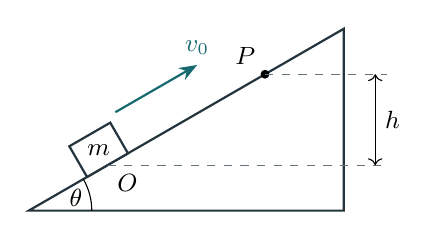
\begin{tikzpicture}
\draw[object] (0,0)--(4,2.309401)--(4,0)--cycle;
\filldraw[object,fill=white,rotate around={30:(1,.57735)}] (.7,.57735) rectangle (1.3,1.02735);
\node at (.8875,.772206) {$m$};\node[below right] at (1,.57735) {$O$};
\draw[motion] (1.1,1.25)--(2.13923,1.85) node[above] {$v_0$};
\draw (.8,0) arc(0:30:.8);\node at (.6,.16) {$\theta$};
\fill (3,1.732051) circle(1.6pt);\node[above left] at (3,1.732051) {$P$};
\draw[guide] (1,.57735)--(4.55,.57735);\draw[guide] (3,1.732051)--(4.55,1.732051);
\draw[<->] (4.4,.57735)--(4.4,1.732051) node[midway,right] {$h$};
\end{tikzpicture}
\figcaption{图 3.3\quad 从初始位置$O$量取竖直高度$h$，$P$表示上滑途中的位置。}
\end{minipage}\end{center}

\workarea

\clearpage

\pdfbookmark[2]{第 4 题 桌孔下落绳的速度与位置}{q4}

\section*{第 4 题\quad 桌孔下落绳的速度与位置}

\tagline{M-03-04}

均匀柔软、不可伸长的绳全长为 $l$，一部分平放在光滑水平桌面上，另一部分经过光滑小孔竖直下垂。初始下垂长度 $0<x_0<l$，整绳从静止下落。设桌上绳已经理顺，各段速率相同，小孔只改变运动方向。求绳速 $v(x)$ 及下端位置 $x(t)$，并说明适用时间。

\begin{center}\begin{minipage}{\linewidth}\centering\begin{tikzpicture}
\draw[object] (-2,1.6)--(-.12,1.6);\draw[object] (.12,1.6)--(1.7,1.6);\draw[traj] (-1.8,1.6)--(0,1.6)--(0,-.8);\node[above right] at (.15,1.6) {$O$};\draw[<->] (.7,-.8)--(.7,1.6) node[midway,right] {$x$};
\end{tikzpicture}
\figcaption{图 3.4\quad 向下量取下垂长度。}
\end{minipage}\end{center}

\workarea

\clearpage

\pdfbookmark[2]{第 5 题 单摆碰钉后的完整圆周与撞钉条件}{q5}

\section*{第 5 题\quad 单摆碰钉后的完整圆周与撞钉条件}

\tagline{M-03-05}

摆长为 $L$ 的单摆，从悬点 $O$ 左侧、与向下竖直方向夹角 $\alpha$ 处静止释放。右侧钉子 $P$ 满足 $OP=r<L$，$OP$ 与向下竖直方向夹角为 $\beta$，其中 $0<\beta<\alpha\leq90^\circ$。绳转到 $OP$ 方向后绕钉运动，绳与钉均理想光滑。求：\begin{enumerate}\item 完成绕钉圆周运动的最小释放角；\item 绳松弛后，小球沿抛物线直接击中钉子 $P$ 所需的释放角。若条件不能实现，应说明。\end{enumerate}

\begin{center}\begin{minipage}{\linewidth}\centering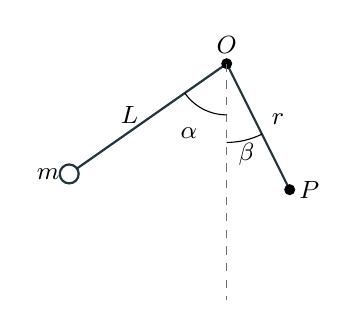
\begin{tikzpicture}
\coordinate(O)at(0,3);\coordinate(P)at(.8,1.4);\coordinate(A)at(-2,1.6);\draw[object] (A)--(O)--(.8,1.4);\fill(O)circle(2pt);\fill(P)circle(2pt);\filldraw[object,fill=white](A)circle(.12);\draw[guide](O)--(0,0);\node[above]at(O){$O$};\node[right]at(P){$P$};\node[left]at(A){$m$};\node[left]at(-1,2.35){$L$};\node[right]at(.45,2.3){$r$};\draw (0,2.35) arc(-90:-145:.65);\node at(-.48,2.12){$\alpha$};\draw (0,2) arc(-90:-63.435:1);\node at(.25,1.85){$\beta$};
\end{tikzpicture}
\figcaption{图 3.5\quad 绳碰钉后，运动半径变为 $a=L-r$。}
\end{minipage}\end{center}

\workarea

\clearpage

\pdfbookmark[2]{第 6 题 圆环双球下滑与悬线张力}{q6}

\section*{第 6 题\quad 圆环双球下滑与悬线张力}

\tagline{M-03-06}

质量 $M$、半径 $R$ 的竖直圆环，用轻细线悬挂。环上串着两个质量均为 $m$ 的光滑小球，从顶端以无限小扰动同时向两侧滑下。$\theta$ 从向上竖直半径量起。\begin{enumerate}\item 假设圆环不动，画出悬线张力 $T$ 随 $x=\cos\theta$ 的曲线，求最小值及对应角度。\item 求圆环可能上升的质量比阈值，画出阈值情形的曲线，并区分“张力为零”与“实际上升”。\end{enumerate}

\begin{center}\begin{minipage}{\linewidth}\centering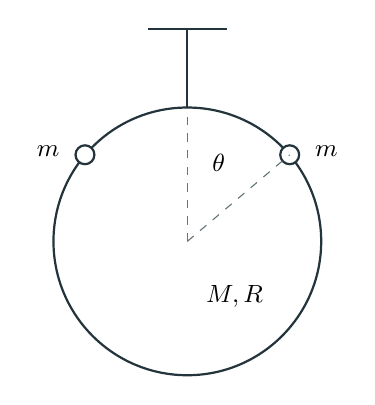
\begin{tikzpicture}
\draw[object](0,0)circle(1.7);\draw[object](0,1.7)--(0,2.7);\draw[object](-.5,2.7)--(.5,2.7);\filldraw[object,fill=white](1.3,1.1)circle(.12);\filldraw[object,fill=white](-1.3,1.1)circle(.12);\draw[guide](0,0)--(0,1.7);\draw[guide](0,0)--(1.3,1.1);\node at(.4,1){$\theta$};\node[right]at(1.5,1.15){$m$};\node[left]at(-1.5,1.15){$m$};\node at(.6,-.7){$M,R$};
\end{tikzpicture}
\figcaption{图 3.6\quad 小球串在环上，可承受环沿径向的推、拉作用。}
\end{minipage}\end{center}

\workarea

\clearpage

\pdfbookmark[2]{第 7 题 滑杆脱离约束后的落点}{q7}

\section*{第 7 题\quad 滑杆脱离约束后的落点}

\tagline{M-03-07}

长 $2r=20\,\mathrm{cm}$ 的理想轻杆，在中心 $C$ 固定质量为 $m$ 的质点。端点 $A$ 靠在光滑竖直墙上，端点 $B$ 支在光滑水平地面上。杆从近似竖直的位置由静止下滑，运动始终在同一竖直平面。按集中质量轻杆模型，求中心 $C$ 第一次触地时距墙角 $O$ 的水平距离。

\begin{center}\begin{minipage}{\linewidth}\centering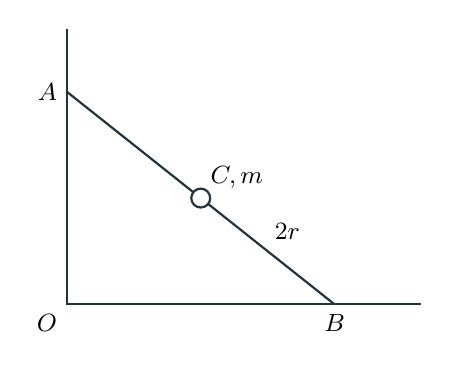
\begin{tikzpicture}
\draw[object](0,3.5)--(0,0)--(4.5,0);\draw[object](0,2.7)--(3.4,0);\filldraw[object,fill=white](1.7,1.35)circle(.12);\node[left]at(0,2.7){$A$};\node[below]at(3.4,0){$B$};\node[above right]at(1.7,1.35){$C,m$};\node[below left]at(0,0){$O$};\node[above]at(2.8,.7){$2r$};
\end{tikzpicture}
\figcaption{图 3.7\quad 两端保持接触时，杆中心沿半径 $r$ 的四分之一圆运动。}
\end{minipage}\end{center}

\workarea

\clearpage

\pdfbookmark[2]{第 8 题 轻杆小球跌落与触地速度}{q8}

\section*{第 8 题\quad 轻杆小球跌落与触地速度}

\tagline{M-03-08}

长 $L$ 的理想轻杆，上端固定一质量为 $m$ 的小球，下端支在粗糙水平地面。由近似竖直位置静止释放，球向右下落。设下端在失去地面支持前不滑动（静摩擦系数足够大），杆的质量可忽略。求球第一次碰地前速度的水平、竖直分量；竖直向上取正。

\begin{center}\begin{minipage}{\linewidth}\centering\begin{tikzpicture}
\draw[object](-.7,0)--(3,0);\draw[object](0,0)--(0,2.7);\filldraw[object,fill=white](0,2.7)circle(.14);\node[left]at(0,1.4){$L$};\node[below]at(0,0){$O$};\draw[motion](.3,2.5)--(1,2.3);\node[right]at(.2,2.7){$m$};
\end{tikzpicture}
\figcaption{图 3.8\quad 初始直立状态取无限小扰动的极限。}
\end{minipage}\end{center}

\workarea

\clearpage

\pdfbookmark[2]{第 9 题 绳绕钉运动与碰钉条件}{q9}

\section*{第 9 题\quad 绳绕钉运动与碰钉条件}

\tagline{M-03-09}

长 $2l$ 的理想细绳，一端固定在钉子 $A$，另一端系小球。小球初始位于 $A$ 右侧同一水平线上，以竖直向下初速度 $v_0$ 运动。钉子 $B$ 位于 $A$ 左侧，$AB=l$。绳转到 $B$ 后，小球绕 $B$ 上行。求小球直接碰到 $A$ 所需的最小初速，允许松绳后以抛体轨迹命中。

\begin{center}\begin{minipage}{\linewidth}\centering\begin{tikzpicture}
\fill(0,0)circle(2pt);\fill(-1.5,0)circle(2pt);\draw[object](0,0)--(3,0);\filldraw[object,fill=white](3,0)circle(.1);\node[above]at(0,0){$A$};\node[above]at(-1.5,0){$B$};\draw[motion](3,0)--(3,-1)node[right]{$v_0$};\draw[guide](3,0)arc(0:-180:3);\draw[<->](-1.5,.65)--(0,.65)node[midway,above]{$l$};
\end{tikzpicture}
\figcaption{图 3.9\quad 先绕 $A$ 经过下半圆，再绕 $B$ 向上运动。}
\end{minipage}\end{center}

\workarea

\clearpage

\pdfbookmark[2]{第 10 题 引力追及中的最大间距}{q10}

\section*{第 10 题\quad 引力追及中的最大间距}

\tagline{M-03-10}

惯性系 $S$ 中，质量分别为 $m_1,m_2$ 的质点 $A,B$ 以万有引力相互吸引。起初 $A$ 静止，间距 $l_0$；$B$ 沿连线远离 $A$，速度 $v_0<\sqrt{2Gm_2/l_0}$。外力 $F$ 始终作用于 $B$，使其速度保持 $v_0$。求两点最大间距及达到该间距前外力在 $S$ 中所做的功。

\begin{center}\begin{minipage}{\linewidth}\centering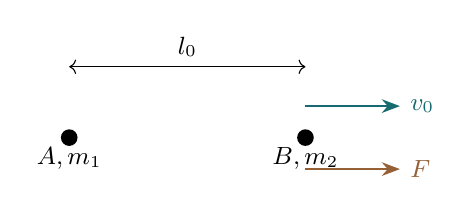
\begin{tikzpicture}
\fill(0,0)circle(3pt);\fill(3,0)circle(3pt);\node[below]at(0,0){$A,m_1$};\node[below]at(3,0){$B,m_2$};\draw[motion](3,.4)--(4.2,.4)node[right]{$v_0$};\draw[force](3,-.4)--(4.2,-.4)node[right]{$F$};\draw[<->](0,.9)--(3,.9)node[midway,above]{$l_0$};
\end{tikzpicture}
\figcaption{图 3.10\quad $F$ 抵消 $B$ 所受引力，$A$ 则不断加速。}
\end{minipage}\end{center}

\workarea

\clearpage

\pdfbookmark[2]{第 11 题 地球直通隧道中的运动}{q11}

\section*{第 11 题\quad 地球直通隧道中的运动}

\tagline{M-03-11}

将地球看作半径 $R$、密度均匀且不自转的球体，地表重力加速度为 $g$。在地表两点 $A,B$ 间开一直通光滑隧道，长度为 $L$。小球从 $A$ 静止释放，忽略空气及其他阻力。求最大速率和首次从 $A$ 到 $B$ 的时间。

\begin{center}\begin{minipage}{\linewidth}\centering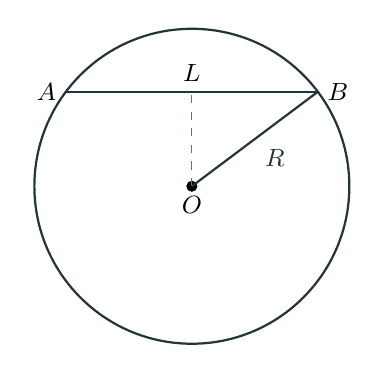
\begin{tikzpicture}
\draw[object](0,0)circle(2);\draw[object](-1.6,1.2)--(1.6,1.2);\fill(0,0)circle(2pt);\node[below]at(0,0){$O$};\node[left]at(-1.6,1.2){$A$};\node[right]at(1.6,1.2){$B$};\draw[guide](0,0)--(0,1.2);\draw[object](0,0)--(1.6,1.2)node[midway,below right]{$R$};\node[above]at(0,1.2){$L$};
\end{tikzpicture}
\figcaption{图 3.11\quad 隧道方向的引力分量指向隧道中点。}
\end{minipage}\end{center}

\workarea

\clearpage

\pdfbookmark[2]{第 12 题 旋转杆上双弹簧小球}{q12}

\section*{第 12 题\quad 旋转杆上双弹簧小球}

\tagline{M-03-12}

两个质量均为 $m$ 的小球串在理想光滑轻杆上，杆绕固定点 $O$ 在水平面内转动。两根相同轻弹簧依次连接 $O$、内球、外球，劲度系数均为 $k$，原长均为 $l_0$。角速度由零无限缓慢增加到 $\omega$，径向瞬态振动可忽略。求外力所做的功、两弹簧长度之比，以及这一准静态分支允许的 $\omega$ 范围。

\begin{center}\begin{minipage}{\linewidth}\centering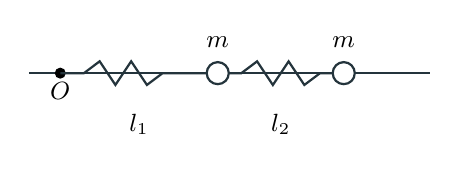
\begin{tikzpicture}
\draw[object](-.4,.2)--(4.7,.2);\fill(0,.2)circle(2pt);\node[below]at(0,.2){$O$};\draw[object](0,.2)--(.3,.2)--(.5,.35)--(.7,.05)--(.9,.35)--(1.1,.05)--(1.3,.2)--(2,.2);\draw[object](2,.2)--(2.3,.2)--(2.5,.35)--(2.7,.05)--(2.9,.35)--(3.1,.05)--(3.3,.2)--(3.6,.2);\filldraw[object,fill=white](2,.2)circle(.14);\filldraw[object,fill=white](3.6,.2)circle(.14);\node[above]at(2,.4){$m$};\node[above]at(3.6,.4){$m$};\node[below]at(1,-.2){$l_1$};\node[below]at(2.8,-.2){$l_2$};
\end{tikzpicture}
\figcaption{图 3.12\quad 外球到转轴的距离为 $l_1+l_2$。}
\end{minipage}\end{center}

\workarea

\clearpage

\pdfbookmark[2]{第 13 题 旋转圆环中的平衡稳定性}{q13}

\section*{第 13 题\quad 旋转圆环中的平衡稳定性}

\tagline{M-03-13}

半径为 $R$ 的光滑竖直圆环，绕其竖直直径以恒定角速度 $\omega$ 转动。质量为 $m$ 的小球串在环上。用从最低点向右量起的有符号角 $\theta$ 表示位置。求相对圆环的平衡位置并讨论稳定性，包含临界角速度的情形。

\begin{center}\begin{minipage}{\linewidth}\centering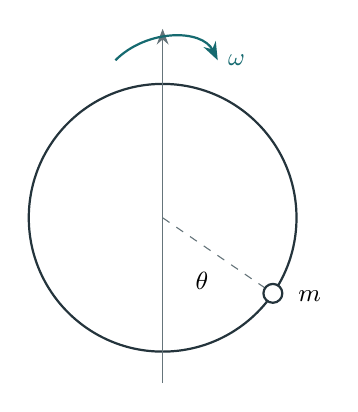
\begin{tikzpicture}
\draw[object](0,0)circle(1.7);\draw[axis](0,-2.1)--(0,2.4);\draw[guide](0,0)--(1.4,-.96);\filldraw[object,fill=white](1.4,-.96)circle(.12);\node[right]at(1.6,-1){$m$};\node at(.5,-.8){$\theta$};\draw[motion](-.6,2)..controls(-.2,2.4)and(.5,2.4)..(.7,2)node[right]{$\omega$};
\end{tikzpicture}
\figcaption{图 3.13\quad 左右对称的非最低点平衡须成对出现。}
\end{minipage}\end{center}

\workarea

\clearpage

\pdfbookmark[2]{第 14 题 弹性小球与移动墙壁}{q14}

\section*{第 14 题\quad 弹性小球与移动墙壁}

\tagline{M-03-14}

质量为 $m$ 的小球在相距 $l$ 的两平行墙壁间，以垂直于墙壁的初速 $v_0$ 往返。墙质量远大于球，碰撞完全弹性，忽略其他作用。\begin{enumerate}\item 两墙固定时，求每壁所受平均力。\item 左壁以 $V\ll v_0$ 缓慢右移，证明在准静态极限中，外力对左壁所做的功等于小球动能增加量。\end{enumerate}

\begin{center}\begin{minipage}{\linewidth}\centering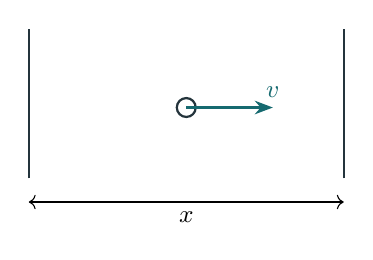
\begin{tikzpicture}
\draw[object](0,-.5)--(0,1.4);\draw[object](4,-.5)--(4,1.4);\filldraw[object,fill=white](2,.4)circle(.12);\draw[motion](2,.4)--(3.1,.4)node[above]{$v$};\draw[<->](0,-.8)--(4,-.8)node[midway,below]{$x$};
\end{tikzpicture}
\figcaption{图 3.14\quad 第二问中，壁距从 $l$ 缩短到 $x$。}
\end{minipage}\end{center}

\workarea

\clearpage

\pdfbookmark[2]{第 15 题 三质点绳系冲量}{q15}

\section*{第 15 题\quad 三质点绳系冲量}

\tagline{M-03-15}

光滑水平面上，静止质点 $A,B,C$ 的质量分别为 $m_1,m_2,m_3$，用两段拉直的理想细绳相连。$\alpha$ 是 $A\to B$ 与 $B\to C$ 两方向的夹角，$0\leq\alpha<90^\circ$。沿 $B\to C$ 方向对 $C$ 施加冲量 $I$。求 $A$ 刚开始运动的速率。

\begin{center}\begin{minipage}{\linewidth}\centering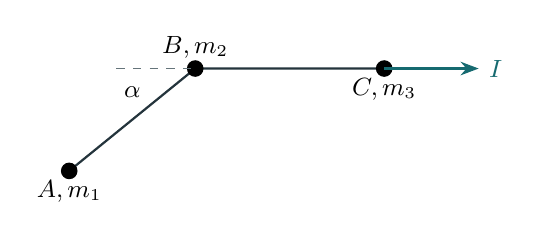
\begin{tikzpicture}
\coordinate(A)at(-1.6,-1.3);\coordinate(B)at(0,0);\coordinate(C)at(2.4,0);\draw[object](A)--(B)--(C);\fill(A)circle(3pt);\fill(B)circle(3pt);\fill(C)circle(3pt);\node[below]at(A){$A,m_1$};\node[above]at(B){$B,m_2$};\node[below]at(C){$C,m_3$};\draw[motion](C)--(3.6,0)node[right]{$I$};\draw[guide](-1,0)--(B);\node at(-.8,-.3){$\alpha$};
\end{tikzpicture}
\figcaption{图 3.15\quad 俯视图；夹角按两条有向绳段的方向定义。}
\end{minipage}\end{center}

\workarea

\clearpage

\pdfbookmark[2]{第 16 题 炮弹最高点爆炸}{q16}

\section*{第 16 题\quad 炮弹最高点爆炸}

\tagline{M-03-16}

炮弹从地面发射，在最高点炸成质量相等的两块。最高点高 $h=19.6\,\mathrm m$，其正下方距发射点 $S_1=1000\,\mathrm m$。第一块在爆炸后 $1.00\,\mathrm s$ 落到该正下方点。忽略空气阻力，取 $g=9.8\,\mathrm{m/s^2}$，求第二块落地点距发射点的水平距离。

\begin{center}\begin{minipage}{\linewidth}\centering\begin{tikzpicture}
\draw[object](-.3,0)--(6,0);\draw[traj](0,0)..controls(.5,1.8)and(1.5,2.4)..(2.2,2.4);\draw[guide](2.2,2.4)--(2.2,0);\fill(2.2,2.4)circle(3pt);\node[above]at(2.2,2.4){爆炸点};\node[below]at(0,0){$O$};\node[below]at(2.2,0){$S_1$};\draw[<->](3,0)--(3,2.4)node[midway,right]{$h$};
\end{tikzpicture}
\figcaption{图 3.16\quad 图示不按水平与竖直距离的实际比例。}
\end{minipage}\end{center}

\workarea

\clearpage

\pdfbookmark[2]{第 17 题 平板车上多人跳离}{q17}

\section*{第 17 题\quad 平板车上多人跳离}

\tagline{M-03-17}

光滑水平地面上，静止平板车质量为 $M$，载有 $N$ 人，每人质量为 $m$。每人向车后跳离，相对于该次跳离后车的速度大小均为 $u$。比较 $N$ 人同时跳离与逐个跳离后，车所得动能的大小。

\begin{center}\begin{minipage}{\linewidth}\centering\begin{tikzpicture}
\draw[object](0,.3)rectangle(4,.6);\draw[object](.6,.15)circle(.15);\draw[object](3.4,.15)circle(.15);\draw[object](-.5,0)--(5,0);\foreach\x in {.8,2,3.2}{\filldraw[object,fill=white](\x,1.1)circle(.15);\draw[object](\x,.95)--(\x,.6);}\node at(2,.43){$M$};\node[above]at(2,1.45){$N$ 人，每人 $m$};
\end{tikzpicture}
\figcaption{图 3.17\quad 向右取车前进的正方向。}
\end{minipage}\end{center}

\workarea

\clearpage

\pdfbookmark[2]{第 18 题 下滑木块中支持力做功}{q18}

\section*{第 18 题\quad 下滑木块中支持力做功}

\tagline{M-03-18}

质量 $M$、倾角 $\theta$ 的斜面体放在光滑水平地面上，质量 $m$ 的木块从斜面顶端高 $h$ 处静止滑至底端。块与斜面之间也光滑。以地面为参考系，求斜面支持力对木块做的功。

\begin{center}\begin{minipage}{\linewidth}\centering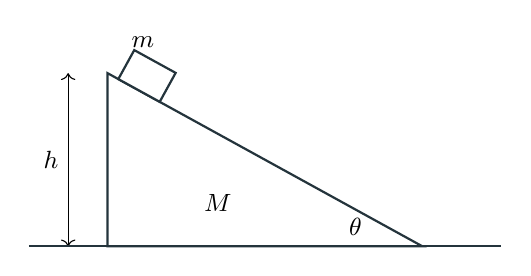
\begin{tikzpicture}
\draw[object](0,0)--(4,0)--(0,2.2)--cycle;\filldraw[object,fill=white,rotate around={-28.81:(.4,1.98)}](.1,1.98)rectangle(.7,2.4);\node at(1.4,.55){$M$};\node[above]at(.45,2.4){$m$};\draw[<->](-.5,0)--(-.5,2.2)node[midway,left]{$h$};\draw[object](-1,0)--(5,0);\node at(3.15,.25){$\theta$};
\end{tikzpicture}
\figcaption{图 3.18\quad 木块相对斜面向右下滑，斜面向左移动。}
\end{minipage}\end{center}

\workarea

\clearpage

\pdfbookmark[2]{第 19 题 半圆槽中小球与木块}{q19}

\section*{第 19 题\quad 半圆槽中小球与木块}

\tagline{M-03-19}

质量 $M$ 的木块放在光滑水平地面上，其上部有半径 $R$ 的光滑半圆凹槽。质量 $m$ 的小球从凹槽右侧最高边缘静止下滑。$\theta$ 为槽心到球的半径与向下竖直方向的夹角，$0\leq\theta\leq\pi/2$。求球的地面速率 $v$、木块向右速率 $V$、球相对槽速率 $w$ 的位置函数；再求球在最低点对槽的压力。

\begin{center}\begin{minipage}{\linewidth}\centering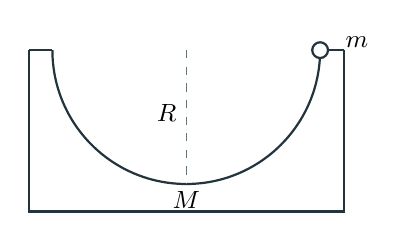
\begin{tikzpicture}
\draw[object](-2,1.7)--(-2,-.35)--(2,-.35)--(2,1.7);\draw[object](-1.7,1.7)arc(180:360:1.7);\draw[object](-2,1.7)--(-1.7,1.7);\draw[object](1.7,1.7)--(2,1.7);\filldraw[object,fill=white](1.7,1.7)circle(.1);\node[right]at(1.9,1.8){$m$};\node at(0,-.2){$M$};\draw[guide](0,1.7)--(0,0);\node[left]at(0,.9){$R$};
\end{tikzpicture}
\figcaption{图 3.19\quad 球从右缘沿凹槽向左下滑。}
\end{minipage}\end{center}

\workarea

\clearpage

\pdfbookmark[2]{第 20 题 非弹性碰撞后弹簧带起木块}{q20}

\section*{第 20 题\quad 非弹性碰撞后弹簧带起木块}

\tagline{M-03-20}

地面上的木块 $m_3$ 通过劲度系数 $k$ 的竖直轻弹簧连接上方木块 $m_2$，初始静止平衡。小球 $m_1$ 从距 $m_2$ 高 $h$ 处静止落下，与 $m_2$ 完全非弹性碰撞并粘住。求使反弹过程中弹簧拉力恰好达到 $m_3g$（离地临界）的最小 $h$。

\begin{center}\begin{minipage}{\linewidth}\centering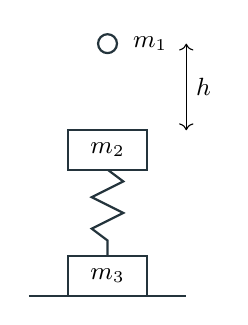
\begin{tikzpicture}
\draw[object](-1,0)--(1,0);\filldraw[object,fill=white](-.5,0)rectangle(.5,.5);\node at(0,.25){$m_3$};\draw[object](0,.5)--(0,.7)--(-.2,.85)--(.2,1.05)--(-.2,1.25)--(.2,1.45)--(0,1.6);\filldraw[object,fill=white](-.5,1.6)rectangle(.5,2.1);\node at(0,1.85){$m_2$};\filldraw[object,fill=white](0,3.2)circle(.12);\node[right]at(.2,3.2){$m_1$};\draw[<->](1,2.1)--(1,3.2)node[midway,right]{$h$};
\end{tikzpicture}
\figcaption{图 3.20\quad 初始弹簧压缩量为 $m_2g/k$。}
\end{minipage}\end{center}

\workarea

\clearpage

\pdfbookmark[2]{第 21 题 滑块弹簧与断绳条件}{q21}

\section*{第 21 题\quad 滑块弹簧与断绳条件}

\tagline{M-03-21}

质量 $M$ 的长滑块静置于光滑水平面，右端用最大承受拉力为 $T_0$ 的理想绳系在墙上，左端固定劲度系数 $k$ 的轻弹簧。质量 $m$ 的小物以向左初速 $v_0$ 在滑块上无摩擦运动，压缩弹簧。约定绳张力达到 $T_0$ 即断裂，断裂本身不消耗能量。求：\begin{enumerate}\item 断绳的最小 $v_0$；\item 断绳后滑块的最大加速度；\item 小物脱离弹簧后，相对桌面的速度为零的条件。\end{enumerate}

\begin{center}\begin{minipage}{\linewidth}\centering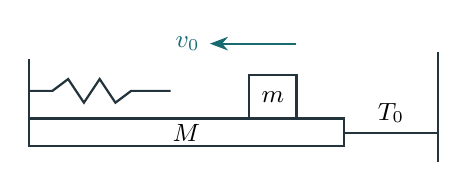
\begin{tikzpicture}
\draw[object](0,0)rectangle(4,.35);\draw[object](0,.35)--(0,1.1);\draw[object](0,.7)--(.3,.7)--(.5,.85)--(.7,.55)--(.9,.85)--(1.1,.55)--(1.3,.7)--(1.8,.7);\filldraw[object,fill=white](2.8,.35)rectangle(3.4,.9);\node at(3.1,.62){$m$};\node at(2,.17){$M$};\draw[object](4,.17)--(5.2,.17);\draw[object](5.2,-.2)--(5.2,1.2);\node[above]at(4.6,.17){$T_0$};\draw[motion](3.4,1.3)--(2.3,1.3)node[left]{$v_0$};
\end{tikzpicture}
\figcaption{图 3.21\quad 弹簧接触只在压缩阶段存在，小物反弹到原长后离开。}
\end{minipage}\end{center}

\workarea

\clearpage

\pdfbookmark[2]{第 22 题 两球与墙的碰撞次数}{q22}

\section*{第 22 题\quad 两球与墙的碰撞次数}

\tagline{M-03-22}

两小球在光滑水平面上沿同一直线运动，质量为 $m_1,m_2$。球 1 以初速 $u>0$ 向右，球 2 起初静止，球 2 右侧有固定弹性墙。球间、球墙的碰撞均完全弹性。求使两球彼此恰好碰撞两次的质量比范围；球墙碰撞不计入“两次”。

\begin{center}\begin{minipage}{\linewidth}\centering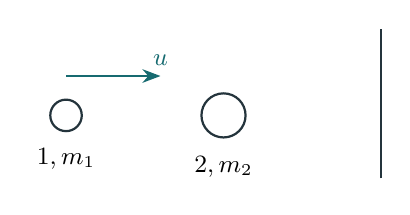
\begin{tikzpicture}
\draw[object](4,-.5)--(4,1.4);\filldraw[object,fill=white](0,.3)circle(.2);\filldraw[object,fill=white](2,.3)circle(.28);\node[below]at(0,0){$1,m_1$};\node[below]at(2,-.1){$2,m_2$};\draw[motion](0,.8)--(1.2,.8)node[above]{$u$};
\end{tikzpicture}
\figcaption{图 3.22\quad 球 2 始终位于球 1 与右墙之间。}
\end{minipage}\end{center}

\workarea

\clearpage

\pdfbookmark[2]{第 23 题 三球铰链杆释放}{q23}

\section*{第 23 题\quad 三球铰链杆释放}

\tagline{M-03-23}

两根长度均为 $l$ 的理想轻杆，在一端用质量 $m$ 的球形铰链连接，另一端分别装质量 $m$ 和 $2m$ 的小球。两端球在光滑水平桌面上，初始两杆近似并拢且竖直，铰链在上，从静止释放后两端球向两侧分开。三球和两杆始终在同一竖直平面。求铰链球碰桌前的速率，以及两杆夹角为 $90^\circ$ 时 $2m$ 球的速率。

\begin{center}\begin{minipage}{\linewidth}\centering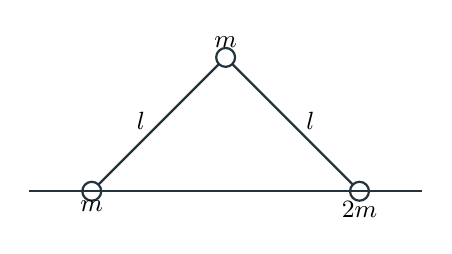
\begin{tikzpicture}
\coordinate(A)at(-1.7,0);\coordinate(B)at(1.7,0);\coordinate(C)at(0,1.7);\draw[object](A)--(C)--(B);\foreach\p in {A,B,C}{\filldraw[object,fill=white](\p)circle(.12);}\draw[object](-2.5,0)--(2.5,0);\node[below]at(A){$m$};\node[below]at(B){$2m$};\node[above]at(C){$m$};\node[left]at(-.9,.9){$l$};\node[right]at(.9,.9){$l$};
\end{tikzpicture}
\figcaption{图 3.23\quad 图示中间状态；两端等高，两杆始终关于铰链所在竖直线几何对称。}
\end{minipage}\end{center}

\workarea

\clearpage

\pdfbookmark[2]{第 24 题 小球反复弹跳总时间}{q24}

\section*{第 24 题\quad 小球反复弹跳总时间}

\tagline{M-03-24}

小球从高 $h$ 处静止下落，与水平地面的恢复系数为 $e$。忽略空气阻力及每次碰撞的持续时间。求从释放到无限次弹跳时间累积终点的总时间，并讨论 $0\leq e\leq1$。

\begin{center}\begin{minipage}{\linewidth}\centering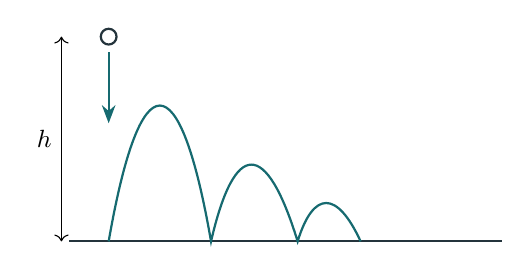
\begin{tikzpicture}
\draw[object](-.5,0)--(5,0);\filldraw[object,fill=white](0,2.6)circle(.1);\draw[motion](0,2.4)--(0,1.5);\draw[<->](-.6,0)--(-.6,2.6)node[midway,left]{$h$};\draw[traj](0,0)..controls(.4,2.3)and(.9,2.3)..(1.3,0)..controls(1.6,1.3)and(2,1.3)..(2.4,0)..controls(2.6,.65)and(2.9,.65)..(3.2,0);
\end{tikzpicture}
\figcaption{图 3.24\quad 弹跳次数以展开示意表示，小球实际始终竖直运动。}
\end{minipage}\end{center}

\workarea

\clearpage

\pdfbookmark[2]{第 25 题 台阶逐级弹跳}{q25}

\section*{第 25 题\quad 台阶逐级弹跳}

\tagline{M-03-25}

台阶每级宽、高均为 $l$，水平踏面光滑。小球逐级向下弹跳，每次反弹后相对本级踏面的最大高度均为 $H$，落点在各级踏面的相同相对位置。小球与踏面的恢复系数为 $0<e<1$，不碰立面。求小球的水平速率及 $H$。

\begin{center}\begin{minipage}{\linewidth}\centering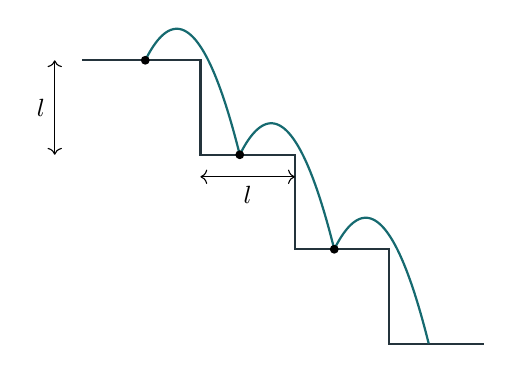
\begin{tikzpicture}
\draw[object] (-.3,3.6)--(1.2,3.6)--(1.2,2.4)--(2.4,2.4)--(2.4,1.2)--(3.6,1.2)--(3.6,0)--(4.8,0);
\foreach \xA/\yA in {.5/3.6,1.7/2.4,2.9/1.2}{
 \draw[traj,domain=0:1,samples=60] plot({\xA+1.2*\x},{\yA+1.2*(2*\x-3*\x^2)});
 \fill (\xA,\yA) circle(1.6pt);}
\draw[<->] (-.65,2.4)--(-.65,3.6) node[midway,left] {$l$};
\draw[<->] (1.2,2.12)--(2.4,2.12) node[midway,below] {$l$};
\end{tikzpicture}
\figcaption{图3.25\quad 等宽等高台阶；示意取$e=1/2$，相邻落点水平、竖直距离均为$l$。}
\end{minipage}\end{center}

\workarea

\clearpage

\pdfbookmark[2]{第 26 题 固定斜面碰撞反弹}{q26}

\section*{第 26 题\quad 固定斜面碰撞反弹}

\tagline{M-03-26}

小球在固定光滑斜面上 $O$ 点正上方 $h=1.60\,\mathrm m$ 处静止释放。斜面向右下方倾斜，倾角 $\theta=15^\circ$，恢复系数 $e=0.60$。忽略空气阻力。求碰后最大上升高度（相对 $O$）、再次撞到斜面的点 $P$ 与 $O$ 的沿面距离，以及碰撞造成的机械能损失百分数。取 $g=9.8\,\mathrm{m/s^2}$。

\begin{center}\begin{minipage}{\linewidth}\centering\begin{tikzpicture}
\draw[object](-1,.267949)--(4,-1.071797);\coordinate(O)at(0,0);\filldraw[object,fill=white](0,2.4)circle(.1);\draw[motion](0,2.2)--(0,1.3)node[right]{$u$};\node[below left]at(O){$O$};\draw[guide](-.5,0)--(1.6,0);\draw (.8,0) arc(0:-15:.8);\node at(.95,-.12){$\theta$};\draw[<->](-.6,0)--(-.6,2.4)node[midway,left]{$h$};
\end{tikzpicture}
\figcaption{图 3.26\quad 碰撞瞬间法向反弹、切向速度不变。}
\end{minipage}\end{center}

\workarea

\clearpage

\pdfbookmark[2]{第 27 题 可动斜面上的斜碰}{q27}

\section*{第 27 题\quad 可动斜面上的斜碰}

\tagline{M-03-27}

质量 $M=2m$ 的斜面体静止在光滑水平桌面上，斜面向右下倾 $\theta=15^\circ$。小球质量为 $m$，从原碰撞点正上方 $h=1.60\,\mathrm m$ 处静止落下，碰撞点距桌面 $H=1.00\,\mathrm m$。斜面光滑，法向相对速度的恢复系数 $e=0.60$，斜面从该点向右延伸至桌面。求碰后两物体的地面速度、小球最高点相对原碰撞点的高度，并判断下一次落在斜面还是桌面。取 $g=9.8\,\mathrm{m/s^2}$。

\begin{center}\begin{minipage}{\linewidth}\centering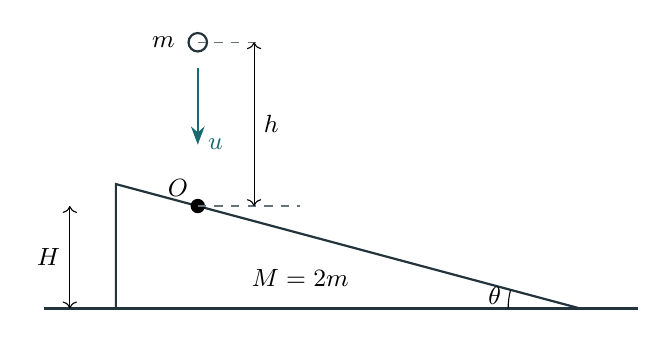
\begin{tikzpicture}[scale=1.3]
\draw[object](-.8,0)--(3.732051,0)--(-.8,1.214359)--cycle;
\draw[object](-1.5,0)--(4.3,0);\node at(1,.3){$M=2m$};
\filldraw[object,fill=white](0,2.6)circle(.09);\node[left]at(-.13,2.6){$m$};
\draw[motion](0,2.35)--(0,1.6)node[right]{$u$};
\fill(0,1)circle(2pt);\node[above left]at(0,1){$O$};
\draw[guide](0,1)--(1,1);\draw[guide](0,2.6)--(.6,2.6);
\draw[<->](-1.25,0)--(-1.25,1)node[midway,left]{$H$};
\draw[<->](.55,1)--(.55,2.6)node[midway,right]{$h$};
\draw (3.032051,0) arc(180:165:.7);\node at(2.9,.12){$\theta$};
\end{tikzpicture}
\figcaption{图3.27\quad 按$15^\circ$绘制斜面；$O$距桌面$H$，球从$O$上方$h$处释放。}
\end{minipage}\end{center}

\workarea

\clearpage

\pdfbookmark[2]{第 28 题 相对平板的反射定律}{q28}

\section*{第 28 题\quad 相对平板的反射定律}

\tagline{M-03-28}

光滑水平桌面上，小球与光滑平板作完全弹性碰撞。平板允许自由平移，不发生转动；碰前可处于任意匀速平移状态。证明：分别用碰前、碰后小球相对平板的速度定义入射角和反射角时，两角相等。角度均从接触面法线量起。

\begin{center}\begin{minipage}{\linewidth}\centering\begin{tikzpicture}
\draw[object](-2,0)--(2,0);\draw[guide](0,-1.6)--(0,1.8);\draw[motion](-1.3,1.3)--(0,0)node[midway,left]{$\vect w_{\mathrm{in}}$};\draw[motion](0,0)--(1.3,1.3)node[midway,right]{$\vect w_{\mathrm{out}}$};\node[below]at(1.7,0){平板};
\end{tikzpicture}
\figcaption{图 3.28\quad 俯视图；两箭头代表相对平板的速度。}
\end{minipage}\end{center}

\workarea

\clearpage

\pdfbookmark[2]{第 29 题 小球在可动圆环内反射}{q29}

\section*{第 29 题\quad 小球在可动圆环内反射}

\tagline{M-03-29}

质量 $M$、半径 $R$ 的均匀光滑圆环静止放在光滑水平桌面上。质点小球质量为 $m$，以地面速度 $v$ 从环上小孔 $H$ 入内，与环内壁完全弹性碰撞 $N\geq1$ 次后，在相对圆环的轨迹上绕一周，再恰好经 $H$ 离开。求入射方向及球、环的出射后地面速度。

\begin{center}\begin{minipage}{\linewidth}\centering\begin{tikzpicture}
\draw[object](0,0)circle(1.8);
\coordinate(H)at(1.8,0);\fill(H)circle(2pt)node[above right]{$H$};
\draw[guide](0,0)--(H);\node[below]at(0,0){$O$};
\draw[motion](2.8,-.5)--(H)node[midway,below]{$v$};
\draw[guide](H)--(.7,.55);
\draw(1.2,0)arc[start angle=180,end angle=153.43495,radius=.6];
\node at(.95,.20){$\theta$};\node at(-.4,2.2){俯视图};
\end{tikzpicture}
\figcaption{图 3.29\quad 入射角 $\theta$ 从 $H\to O$ 的内法线量起。}
\end{minipage}\end{center}

\workarea

\clearpage

\pdfbookmark[2]{第 30 题 三质点万有引力相对平衡}{q30}

\section*{第 30 题\quad 三质点万有引力相对平衡}

\tagline{M-03-30}

质量分别为 $m_1,m_2,m_3$ 的三质点，只通过万有引力相互作用，以共同角速度 $\omega$ 绕通过质心、垂直于它们所在平面的轴转动。求保持相对位置不变的条件。先讨论三点不共线的情形，再说明共线情形是否可能。

\begin{center}\begin{minipage}{\linewidth}\centering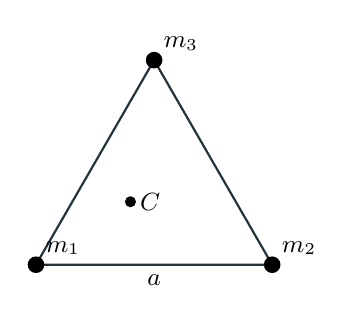
\begin{tikzpicture}
\coordinate(A)at(0,0);\coordinate(B)at(3,0);\coordinate(D)at(1.5,2.598);\draw[object](A)--(B)--(D)--cycle;\foreach\p/\lab in {A/1,B/2,D/3}{\fill(\p)circle(3pt);\node[above right]at(\p){$m_\lab$};}\fill(1.2,.8)circle(2pt);\node[right]at(1.2,.8){$C$};\node[below]at(1.5,0){$a$};
\end{tikzpicture}
\figcaption{图 3.30\quad 质心一般不在几何中心；等边图示对应非共线解。}
\end{minipage}\end{center}

\workarea

\clearpage

\pdfbookmark[2]{第 31 题 等功跳车的动能比较}{q31}

\section*{第 31 题\quad 等功跳车的动能比较}

\tagline{M-03-31}

静止平板车质量为 $M$，光滑地面上的车载 $N$ 人，每人质量为 $m$。每人以相同的功 $w$ 向车后跳离，假设这些功都转化为车和人的平动动能，不计耗散及转动。怎样安排跳法能使车最终动能最大？求该最大值。

\begin{center}\begin{minipage}{\linewidth}\centering\begin{tikzpicture}
\draw[object](0,.3)rectangle(4,.6);\draw[object](.6,.15)circle(.15);\draw[object](3.4,.15)circle(.15);\draw[object](-.5,0)--(5,0);\foreach\x in {.8,2,3.2}{\filldraw[object,fill=white](\x,1.1)circle(.15);\draw[object](\x,.95)--(\x,.6);}\node at(2,.43){$M$};\node[above]at(2,1.45){$N$ 人，每人 $m$};
\end{tikzpicture}
\figcaption{图 3.31\quad 本题固定每人的功，区别于第 17 题固定相对跳速。}
\end{minipage}\end{center}

\workarea

\clearpage

\pdfbookmark[2]{第 32 题 子弹射入弹簧连接木块}{q32}

\section*{第 32 题\quad 子弹射入弹簧连接木块}

\tagline{M-03-32}

光滑水平面上，质量 $m_1,m_2$ 的木块用劲度系数 $k$ 的轻弹簧相连，起初静止且弹簧为原长。子弹质量 $m$，以水平向右初速 $v_0$ 射入 $m_1$ 并嵌住，射入时间极短。求随后弹簧的最大压缩量，以及 $m_2$ 相对地面的最大、最小速度。

\begin{center}\begin{minipage}{\linewidth}\centering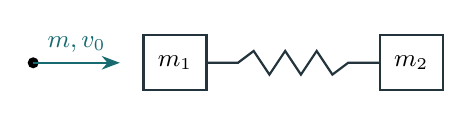
\begin{tikzpicture}
\filldraw[object,fill=white](0,0)rectangle(.8,.7);\filldraw[object,fill=white](3,0)rectangle(3.8,.7);\node at(.4,.35){$m_1$};\node at(3.4,.35){$m_2$};\draw[object](.8,.35)--(1.2,.35)--(1.4,.5)--(1.6,.2)--(1.8,.5)--(2,.2)--(2.2,.5)--(2.4,.2)--(2.6,.35)--(3,.35);\fill(-1.4,.35)circle(2pt);\draw[motion](-1.4,.35)--(-.3,.35)node[midway,above]{$m,v_0$};
\end{tikzpicture}
\figcaption{图 3.32\quad 碰撞瞬间弹簧长度来不及改变，第二块尚无速度。}
\end{minipage}\end{center}

\workarea

\clearpage

\pdfbookmark[2]{第 33 题 箱中滑块多次碰撞}{q33}

\section*{第 33 题\quad 箱中滑块多次碰撞}

\tagline{M-03-33}

质量为 $m$ 的箱子起初静止于光滑水平地面，箱内底面光滑，有质量同为 $m$ 的质点滑块。滑块以水平初速 $v_0$ 向右运动，与两内壁反复碰撞，恢复系数 $e=2^{-1/4}$，碰撞时间可略。\begin{enumerate}\item 最多碰撞几次，系统总动能损失仍不大于初始动能的 $40\%$？\item 箱内宽度为 $L$，滑块初始距左壁 $x_0$，求从开始到完成上述次数的碰撞时箱子的平均速度，并给出 $x_0=0$ 的结果。\end{enumerate}

\begin{center}\begin{minipage}{\linewidth}\centering\begin{tikzpicture}
\draw[object](0,0)rectangle(4,1.3);\filldraw[object,fill=white](.1,.1)rectangle(.7,.7);\node at(.4,.4){$m$};\node[above]at(2,1.3){箱子质量 $m$};\draw[motion](.8,.6)--(1.9,.6)node[above]{$v_0$};\draw[<->](0,-.4)--(4,-.4)node[midway,below]{$L$};
\end{tikzpicture}
\figcaption{图 3.33\quad 图示滑块从左壁附近向右；第二问保留一般初始位置。}
\end{minipage}\end{center}

\workarea

\clearpage

\pdfbookmark[2]{第 34 题 核反应阈能}{q34}

\section*{第 34 题\quad 核反应阈能}

\tagline{M-03-34}

动能为 $E_0$ 的 $^{4}\mathrm{He}$ 核轰击静止的 $^{7}\mathrm{Li}$ 核，先形成复合核，再分裂为 $^{10}\mathrm B$ 和中子 $^{1}\mathrm n$。反应吸收能量 $Q=2.8\,\mathrm{MeV}$。采用非相对论近似，各核惯性质量按质量数之比 $4:7:10:1$ 取值，忽略质量亏损对平动质量的修正。求反应所需最小 $E_0$，及阈值处中子的实验室动能。

\begin{center}\begin{minipage}{\linewidth}\centering\begin{tikzpicture}
\node[draw,circle]at(0,0){$^4\mathrm{He}$};\node[draw,circle]at(3,0){$^7\mathrm{Li}$};\draw[motion](.6,0)--(2.3,0)node[midway,above]{$E_0$};\node at(3,-1){靶核静止};\node[align=left]at(6,0){$^{10}\mathrm B+{}^1\mathrm n$\\吸收 $Q$};
\end{tikzpicture}
\figcaption{图 3.34\quad 阈值由可用于相对运动的动能决定。}
\end{minipage}\end{center}

\workarea

\clearpage

\pdfbookmark[2]{第 35 题 变质量物体方程}{q35}

\section*{第 35 题\quad 变质量物体方程}

\tagline{M-03-35}

一主体作直线运动，质量 $M(t)$、地面速度 $v(t)$ 随时间变化。以 $u$ 表示加入质量进入前，或流出质量离开后的地面速度，$F$ 为主体所受合外力。用短时间内质量固定的扩展系统证明
\[
M\frac{\dd v}{\dd t}=(u-v)\frac{\dd M}{\dd t}+F.
\]
质量流只在边界处交换动量，外力场有限。

\begin{center}\begin{minipage}{\linewidth}\centering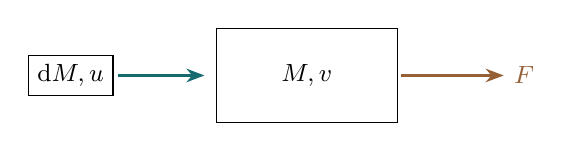
\begin{tikzpicture}
\node[draw,minimum width=2.3cm,minimum height=1.2cm]at(1,0){$M,v$};\node[draw]at(-2,0){$\dd M,u$};\draw[motion](-1.4,0)--(-.3,0);\draw[force](2.2,0)--(3.5,0)node[right]{$F$};
\end{tikzpicture}
\figcaption{图 3.35\quad 图示流入情形；扩展系统包含主体与即将流入的质量。}
\end{minipage}\end{center}

\workarea

\clearpage

\pdfbookmark[2]{第 36 题 下落绳子的变质量分析}{q36}

\section*{第 36 题\quad 下落绳子的变质量分析}

\tagline{M-03-36}

均匀柔软绳全长 $l$，初始竖直静止，下端刚接触地面，释放后下落。采用理想沉积模型：未落地部分自由落体；落地微段立即停止且不反弹，堆积不向未落地部分传递附加拉力，堆积高度可忽略。证明下落过程中地面压力为已落地绳重的三倍，并说明最后完全落地后的变化。

\begin{center}\begin{minipage}{\linewidth}\centering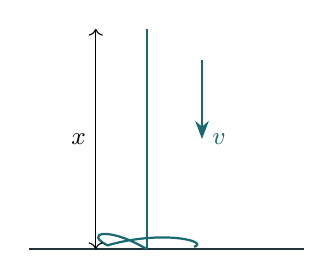
\begin{tikzpicture}
\draw[object](-1.5,0)--(2,0);\draw[traj](0,0)--(0,2.8);\draw[traj](0,0)..controls(-.5,.3)and(-.8,.2)..(-.5,.05)..controls(.2,.25)and(.8,.1)..(.6,.03);\draw[motion](.7,2.4)--(.7,1.4)node[right]{$v$};\draw[<->](-.65,0)--(-.65,2.8)node[midway,left]{$x$};
\end{tikzpicture}
\figcaption{图 3.36\quad 剩余悬空长度 $x$，落地长度 $s=l-x$。}
\end{minipage}\end{center}

\workarea

\clearpage

\pdfbookmark[2]{第 37 题 火箭竖直发射}{q37}

\section*{第 37 题\quad 火箭竖直发射}

\tagline{M-03-37}

火箭从地面静止竖直发射，干质量为 $M_s$，初始燃料质量 $M_f$。燃气相对火箭向下喷出，速率恒为 $c>0$，质量消耗率恒为 $b>0$。重力加速度 $g$ 恒定，无空气阻力，且 $bc>(M_s+M_f)g$，点火即可离地。求推力、加速度、燃烧期任意时刻的速度和高度，燃尽瞬间各量，以及最大高度和从发射到最高点的时间。

\begin{center}\begin{minipage}{\linewidth}\centering\begin{tikzpicture}
\draw[object](-.5,0)--(1.5,0);\draw[object](0,.5)--(0,2.2)--(.4,2.8)--(.8,2.2)--(.8,.5)--cycle;\draw[motion](.4,.4)--(.4,-.8)node[right]{$c$（相对）};\draw[motion](1.5,1)--(1.5,2.2)node[right]{$v$};\node[right]at(1, .6){$M_s+M_f-bt$};
\end{tikzpicture}
\figcaption{图 3.37\quad 燃气相对喷速用正的速率 $c$ 表示，方向另行指定。}
\end{minipage}\end{center}

\workarea

\clearpage

\pdfbookmark[2]{第 38 题 小球带绳竖直上抛}{q38}

\section*{第 38 题\quad 小球带绳竖直上抛}

\tagline{M-03-38}

质量为 $m$ 的小球下系足够长、线密度为 $\lambda$ 的均匀柔绳，绳初始松放在地面。小球以初速度 $v_0$ 从地面竖直上抛，依次将静止绳段带起。理想化为已离地绳竖直且各段与球同速，新进入绳段在被带起前静止，拾取时无反弹，忽略阻力。求上升速率随高度 $x$ 的规律及最大高度。

\begin{center}\begin{minipage}{\linewidth}\centering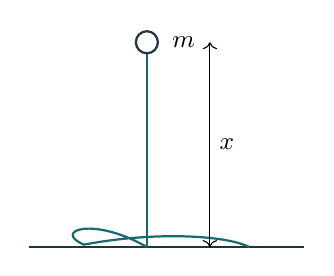
\begin{tikzpicture}
\draw[object](-1.5,0)--(2,0);\draw[traj](0,0)--(0,2.6);\filldraw[object,fill=white](0,2.6)circle(.14);\node[right]at(.2,2.6){$m$};\draw[traj](0,0)..controls(-.7,.4)and(-1.2,.2)..(-.8,.03)..controls(.1,.2)and(1,.15)..(1.3,0);\draw[<->](.8,0)--(.8,2.6)node[midway,right]{$x$};
\end{tikzpicture}
\figcaption{图 3.38\quad 运动主体质量为 $m+\lambda x$。}
\end{minipage}\end{center}

\workarea

\clearpage

\pdfbookmark[2]{第 39 题 雾中水滴变质量下落}{q39}

\section*{第 39 题\quad 雾中水滴变质量下落}

\tagline{M-03-39}

球形水滴在静止、密度均匀的雾中下落，吸收其扫过截面内全部雾水。水滴始终球形，水的密度为常量 $\rho_w$，雾中可被收集的水质量密度为 $\rho_f>0$。初始半径有限且为正，初始向下速度有限且非负。忽略空气黏滞阻力，$g$ 恒定。证明长时间后加速度趋于常量，并求该常量。

\begin{center}\begin{minipage}{\linewidth}\centering\begin{tikzpicture}
\filldraw[object,fill=accent!8](0,1.5)circle(.55);\draw[guide](-.55,-.8)--(-.55,1.5);\draw[guide](.55,-.8)--(.55,1.5);\draw[motion](0,.7)--(0,-.5)node[right]{$v$};\draw[<->](0,1.5)--(.55,1.5)node[midway,above]{$r$};\foreach\p in {(-1,0),(1,.4),(-.8,2.5),(1,2.2),(.3,-.9)}{\fill[color=muted]\p circle(1pt);}\node at(2,1.2){静止雾水};
\end{tikzpicture}
\figcaption{图 3.39\quad 吸收率由迎面截面积 $\pi r^2$ 决定。}
\end{minipage}\end{center}

\workarea

\end{document}
